\documentclass[12pt,letterpaper,twoside]{article}

% ================== CODIFICACIÓN Y LENGUAJE ==================
\usepackage[T1]{fontenc}
\usepackage[spanish,es-nodecimaldot]{babel}
\usepackage{lmodern}

% ================== MATEMÁTICAS ==================
\usepackage{amsmath,amssymb,mathtools}

% ================== GRÁFICOS Y FIGURAS ==================
\usepackage{graphicx}
\usepackage{float}
\usepackage{caption}
\usepackage{circuitikz}

% ================== TABLAS ==================
\usepackage{array}
\usepackage{booktabs}

% ================== UNIDADES ==================
\usepackage{siunitx}

% ================== LISTAS ==================
\usepackage{enumitem}

% ================== TEXTO Y FORMATO ==================
\usepackage{textcomp}
\usepackage{multicol}
\usepackage[usenames,dvipsnames]{xcolor}

% ================== HIPERVÍNCULOS ==================
\usepackage[
    colorlinks=true,
    pdfstartview=FitV,
    linkcolor=black,
    citecolor=blue,
    urlcolor=blue
]{hyperref}

% ================== CÓDIGO (ESTILO IDE) ==================
\usepackage{listings}

\lstdefinestyle{mystyle}{
    backgroundcolor=\color{gray!10},
    commentstyle=\color{green!50!black},
    keywordstyle=\color{blue},
    stringstyle=\color{orange},
    numberstyle=\tiny\color{gray},
    basicstyle=\ttfamily\small,
    breaklines=true,
    numbers=left,
    numbersep=5pt,
    frame=single,
    tabsize=2,
    captionpos=b,
    showstringspaces=false,
    showspaces=false,
    showtabs=false,
    columns=fullflexible,
    keepspaces=true
}

\lstset{style=mystyle}

% ================== CONFIGURACIÓN DE PÁGINA ==================
\usepackage[
    letterpaper,
    left=2.5cm,
    right=2.5cm,
    top=2.5cm,
    bottom=2.5cm
]{geometry}

\setlength{\headsep}{10mm}
\setlength{\parindent}{2pc}
\setlength{\columnsep}{10mm}
\setlength{\parskip}{0.2ex}

% ================== ENCABEZADOS ==================
\usepackage{fancyhdr}

\pagestyle{fancy}
\addtolength{\headheight}{4pt}
\renewcommand{\sectionmark}[1]{\markboth{#1}{}}

\fancyhf{}
\fancyhead[LE,RO]{\thepage}
\fancyhead[RE]{\small Producto Integrador del Aprendizaje}
\fancyhead[LO]{\leftmark}
\renewcommand{\headrulewidth}{0.4pt}

\fancypagestyle{plain}{
\fancyhf{}
\renewcommand{\headrulewidth}{0pt}
\renewcommand{\footrulewidth}{0pt}
}

% ================== AJUSTES EN ESPAÑOL ==================
\addto\captionsspanish{
  \renewcommand{\tablename}{Tabla}
}

\begin{document}

\setlength{\parskip}{0.5em}

 \input{Plantilla/Guionado}

\pagenumbering{roman}
\thispagestyle{empty}

\begin{Large}
    \begin{center}
        \Large \textbf{Universidad Autónoma de Nuevo León}\\
        \large \textbf{Facultad de Ingeniería Mecánica y Eléctrica}
    \end{center}
\end{Large}

\newcommand{\logoheight}{3.0cm}

\begin{center}
  \begin{minipage}[c]{0.45\linewidth}\centering
    
\includegraphics[height=\logoheight]{Imagenes/UANL.png}
  \end{minipage}
  \hfill
  \begin{minipage}[c]{0.45\linewidth}\centering
    
\includegraphics[height=\logoheight]{Imagenes/logo_fime.jpg}
  \end{minipage}
\end{center}

\vspace{0.6\baselineskip}

\begin{center}
\large
    {Unidad de aprendizaje:}
\end{center}
\begin{center}
\Large
    \textbf{Control Óptimo}\\
\end{center}

\begin{Large}
    \newlength{\longTitulo}
    \settowidth{\longTitulo}{\textbf{xxxxxxxxxxxxxxxxxxxxxxxxxxxxxxxxxxxxxxxxxxxxxxxx}}
    \begin{center}
        \rule{\longTitulo}{.5mm}\\
        \large{Producto Integrador de Aprendizaje (PIA)} \\ 
        \Large{\textbf{Diseño e implementación de un control óptimo}}\\
        \rule{\longTitulo}{.5mm}\\
    \end{center}
\end{Large}

\begin{center}
\normalsize{que se presenta como parte de la}\\
\Large{\textbf{Actividad fundamental 3}}\\
\end{center}

\begin{center}
\normalsize{Docente:} \\ 
M. C. Miguel Cabrera Quiroz\\
\end{center}

\begin{center}
    {Presenta:}\\
\large{\textbf{González Alvarez Gabriel}}
\end{center}

\begin{center}
\normalsize
\begin{tabular}{rl}
Matrícula: & 2109326 \\[0.3cm]
Grupo: & 003 \\[0.3cm]
Días: & Lunes, Miércoles y Viernes\\[0.3cm]
Hora: & N5 \\[0.3cm]
Aula: & 3108 \\[0.3cm]
Fecha de entrega final: & 29 de mayo de 2026
\end{tabular}
\end{center}

\vfill

\begin{center}
    {Ciudad Universitaria, San Nicolás de los Garza, Nuevo León.}
\end{center}

\newpage

\tableofcontents
\vfill
\textbf{ }
\vfill

\pagenumbering{arabic}
\setcounter{page}{1}
\renewcommand{\labelitemi}{$\checkmark$}

\newpage

% =========================================================
\section{Introducción}

En el presente trabajo se desarrolla el modelado matemático de un sistema eléctrico compuesto por una red de resistencias y capacitores, con el propósito de analizar su comportamiento dinámico y diseñar distintas estrategias de control basadas en técnicas de control moderno.

A partir del circuito propuesto, se obtienen las ecuaciones diferenciales que describen el sistema mediante la aplicación de las leyes de Kirchhoff. Posteriormente, dichas ecuaciones se expresan en forma de espacio de estados, considerando como variables de estado los voltajes en los capacitores.

Con base en este modelo, se define un índice de desempeño que permite evaluar el comportamiento del sistema en términos del seguimiento de la salida y el esfuerzo de control. A partir de este criterio se desarrolla un controlador óptimo LQR mediante la solución de la ecuación algebraica de Riccati.

De manera adicional, se implementan estrategias de control mediante asignación de polos, control integral por asignación de polos y control óptimo con acción integral (LQI), permitiendo comparar experimentalmente el desempeño de distintos enfoques de control bajo condiciones equivalentes.

Asimismo, se plantea una estrategia de prealimentación mediante el cálculo de una ganancia \(g\), con el objetivo de garantizar el seguimiento de una referencia constante sin error en estado estacionario.

Finalmente, se desarrolla una implementación experimental utilizando un microcontrolador ESP32 y múltiples plantas RC físicamente equivalentes, lo que permite validar el comportamiento de los controladores mediante mediciones en tiempo real y comparar su desempeño respecto al índice de desempeño definido.

Este enfoque integra el modelado físico del sistema, el diseño de controladores y la validación experimental, proporcionando una base sólida para el análisis e implementación de estrategias de control moderno.

% =========================================================
\section{Modelo del sistema}

El sistema bajo estudio corresponde a una red eléctrica compuesta por resistencias y capacitores. En la Figura \ref{fig:circuito} se muestra el circuito equivalente.

\begin{figure}[H]
\centering
\begin{circuitikz}[american]
\draw (0,0) node[ground]{} 
to[V, l=$u(t)$] (0,4)
to[R, l=$R_1$, i>^=$q_1$] (3,4)
node[circ]{} node[above]{$V_1$}
to[C, l_=$C_1$, i>^=$q_{C1}$] (3,0)
node[ground]{}

(3,4) to[R, l=$R_2$, i>^=$q_2$] (6,4)
node[circ]{} node[above]{$V_2$}
to[C, l_=$C_2$, i>^=$q_{C2}$] (6,0)
node[ground]{}

(6,4) to[R, l=$R_3$, i>^=$q_3$] (9,4)
-- (9,0) node[ground]{};
\end{circuitikz}
\caption{Circuito RC del sistema}
\label{fig:circuito}
\end{figure}

Aplicando la Ley de Corrientes de Kirchhoff:

\begin{align}
\frac{u - V_1}{R_1} &= C_1 \frac{dV_1}{dt} + \frac{V_1 - V_2}{R_2} \\[10pt]
\frac{V_1 - V_2}{R_2} &= C_2 \frac{dV_2}{dt} + \frac{V_2}{R_3}
\end{align}

Definiendo:

\begin{equation}
x_1 = V_1, \quad x_2 = V_2, \quad y = x_2
\end{equation}

Se obtienen las ecuaciones de estado:

\begin{align}
\dot{x}_1 &= \left( - \frac{1}{R_1 C_1} - \frac{1}{R_2 C_1} \right)x_1 
+ \frac{1}{R_2 C_1}x_2 
+ \frac{1}{R_1 C_1}u \\[10pt]
\dot{x}_2 &= \frac{1}{R_2 C_2}x_1 
- \left( \frac{1}{R_2 C_2} + \frac{1}{R_3 C_2} \right)x_2
\end{align}

Forma matricial:

\begin{equation}
\begin{bmatrix}
\dot{x}_1 \\
\dot{x}_2
\end{bmatrix}
=
\begin{bmatrix}
-\frac{1}{R_1 C_1} - \frac{1}{R_2 C_1} & \frac{1}{R_2 C_1} \\
\frac{1}{R_2 C_2} & -\frac{1}{R_2 C_2} - \frac{1}{R_3 C_2}
\end{bmatrix}
\begin{bmatrix}
x_1 \\
x_2
\end{bmatrix}
+
\begin{bmatrix}
\frac{1}{R_1 C_1} \\
0
\end{bmatrix}
u
\label{eq:ss}
\end{equation}

\begin{equation}
y =
\begin{bmatrix}
0 & 1
\end{bmatrix}
\begin{bmatrix}
x_1 \\
x_2
\end{bmatrix}
\label{eq:salida}
\end{equation}

% =========================================================
\section{Índice de desempeño}
\label{sec:performance}

Con el objetivo de diseñar un controlador óptimo, se define un índice de desempeño que permite evaluar la calidad de la respuesta del sistema. Este índice se plantea como:

\begin{equation}
J = \int_{0}^{\infty} \left( x^T(t) Q x(t) + u^T(t) R u(t) \right) dt
\end{equation}

donde \(Q\) es una matriz de ponderación de estados y \(R\) es una ponderación asociada al esfuerzo de control.

La formulación anterior corresponde al problema de regulación cuadrática lineal, abordado en textos clásicos de control óptimo y control moderno \cite{Ogata,Kirk}.

Dado que se desea dar mayor importancia al seguimiento del voltaje en el capacitor 2, se establece que dicho estado tenga un peso mayor. Por lo tanto, la matriz \(Q\) se define como:

\begin{equation}
Q =
\begin{bmatrix}
1 & 0 \\
0 & 5
\end{bmatrix}
\end{equation}

Por otro lado, \(R\) se selecciona como un escalar positivo que penaliza el uso excesivo de la señal de control:

\begin{equation}
R = 1
\end{equation}

Este planteamiento permite balancear el compromiso entre el desempeño del sistema y el esfuerzo requerido por el actuador.

% =========================================================
\section{Solución numérica}

El problema de optimización se resolvió mediante la solución de la ecuación algebraica de Riccati asociada al problema de regulación cuadrática lineal descrito en \cite{Kirk}, utilizando Python. El código completo se presenta en el Apéndice \ref{sec:SolveLQR}. A continuación se muestran las líneas relevantes correspondientes al cálculo de la solución de Riccati y la ganancia LQR:

\begin{lstlisting}[language=Python, caption={Cálculo de la ganancia LQR}, firstnumber=25]
P = solve_continuous_are(A,B,Q,R)
\end{lstlisting}

\begin{lstlisting}[language=Python, caption={Cálculo de la ganancia LQR (continuación)}, firstnumber=30]
K = np.linalg.inv(R) @ B.T @ P
\end{lstlisting}

Se obtuvo:

\[
K = \begin{bmatrix} 0.41421356 & 0.41421356 \end{bmatrix}
\]

De manera adicional, se desarrollaron estrategias de control mediante asignación de polos, control integral por asignación de polos y control óptimo con acción integral (LQI), con el propósito de comparar experimentalmente su desempeño respecto al controlador LQR.

En el caso del controlador LQI, el sistema fue aumentado incorporando un estado integral asociado al error de seguimiento, resolviendo posteriormente la ecuación algebraica de Riccati mediante el mismo procedimiento utilizado para el LQR convencional.

Por otro lado, los controladores basados en asignación de polos emplean un observador de estados para estimar el voltaje asociado al primer capacitor, debido a que únicamente se mide directamente la salida del sistema. El desarrollo matemático del observador y de las estrategias de control implementadas se presenta en el Apéndice \ref{sec:Controladores}.

Asimismo, el código correspondiente a la solución numérica del controlador LQI mediante Python se presenta en el Apéndice \ref{sec:SolveLQI}.

% =========================================================
\section{Seguimiento de referencia mediante cambio de coordenadas}

Para garantizar el seguimiento de una referencia constante sin error en estado estacionario, se emplea un enfoque basado en cambio de coordenadas, el cual permite transformar el problema de seguimiento en uno de regulación. 

Bajo este enfoque, la ley de control se plantea como:

\begin{equation}
u = -Kx + g r
\end{equation}

donde \(K\) es la ganancia de retroalimentación de estados y \(g\) es una ganancia de ajuste encargada de asegurar el valor deseado en estado estacionario.

\begin{equation}
g =
\begin{bmatrix}
K & 1
\end{bmatrix}
\begin{bmatrix}
A & B \\
C & D
\end{bmatrix}^{-1}
\begin{bmatrix}
0 \\
0 \\
1
\end{bmatrix}
\end{equation}

donde \(K = \begin{bmatrix} k_1 & k_2 \end{bmatrix}\) y las matrices corresponden al modelo definido en (\ref{eq:ss}) y (\ref{eq:salida}).

La matriz aumentada es:

\begin{equation}
\begin{bmatrix}
A & B \\
C & D
\end{bmatrix}
=
\begin{bmatrix}
-\frac{1}{R_1 C_1} - \frac{1}{R_2 C_1} & \frac{1}{R_2 C_1} & \frac{1}{R_1 C_1} \\
\frac{1}{R_2 C_2} & -\frac{1}{R_2 C_2} - \frac{1}{R_3 C_2} & 0 \\
0 & 1 & 0
\end{bmatrix}
\end{equation}

Finalmente, al realizar las operaciones correspondientes, se obtiene:

\begin{equation}
g = k_1 + k_2 + \frac{k_1 R_2 + R_1 + R_2}{R_3} +1
\end{equation}

Esta expresión se utilizó para calcular la ganancia de prealimentación del controlador LQR, cuyo código completo se presenta en el Apéndice \ref{sec:esp32}, correspondiente a la implementación en el microcontrolador. En particular, la instrucción correspondiente se muestra a continuación:

\begin{lstlisting}[language=C++, firstnumber=152, caption={Cálculo de la ganancia de seguimiento para el controlador LQR}]
  Kp_3 = K1_3 + K2_3 + 1 + (K1_3*R2+R1+R2)/R3;  //Ganancia de seguimiento mediante cambio de coordenadas
\end{lstlisting}

Esta ganancia permite garantizar que la salida del sistema siga la referencia deseada sin error en estado estacionario, siempre que el modelo represente adecuadamente la dinámica del sistema.

La estrategia de seguimiento mediante prealimentación y cambio de coordenadas empleada en este trabajo corresponde al enfoque clásico presentado en \cite{Ogata}.

% =========================================================
\section{Implementación en microcontrolador}

La ley de control implementada es:

\[
u = -Kx + gr
\]

El fragmento principal del código correspondiente a esta ley se muestra en el Código \ref{lst:lqr}, 
mientras que el programa completo del microcontrolador se presenta en el Apéndice \ref{sec:esp32}.

El programa completo implementado en el ESP32 incluye las cuatro estrategias de control evaluadas experimentalmente: asignación de polos, control integral por asignación de polos, control óptimo LQR y control con acción integral (LQI). 

\begin{lstlisting}[language=C++, firstnumber=225, caption={Control LQR implementado}, label={lst:lqr}]
// ===== Control LQR =====
void control_3(){
  X13 = analogRead(X1_3)*mX;  //estado 1
  X23 = analogRead(X2_3)*mX;  //estado 2
  Y3 = X23;  //salida
  //Ley de control u = -Kx
  U3 = Kp_3*R - K1_3*X13 - K2_3*X23;

  U3 = constrain(U3,0,3.3);  //saturacion
 }
\end{lstlisting}

Donde \(x_1\) y \(x_2\) corresponden a los voltajes medidos en cada capacitor del sistema.

En las estrategias basadas en asignación de polos se empleó un observador de estados de orden completo para estimar el voltaje correspondiente al estado \(x_1\), utilizando únicamente la medición directa de la salida del sistema. 

Por otro lado, en las implementaciones LQR y LQI se realizó la medición directa de ambos estados, por lo que no fue necesario utilizar estimación mediante observador. El desarrollo y código completo del observador implementado se presentan en el Apéndice \ref{sec:observador}.

% =========================================================
\section{Implementación experimental}

Con el objetivo de validar experimentalmente el modelo desarrollado y comparar distintas estrategias de control bajo condiciones equivalentes, se realizó la implementación física del sistema utilizando una tarjeta de pruebas (protoboard) y un microcontrolador ESP32.

El circuito RC descrito previamente en la Figura \ref{fig:circuito} fue replicado en cuatro ocasiones dentro de la misma tarjeta, empleando valores idénticos de resistencias y capacitores para cada configuración. Esta disposición permite ejecutar múltiples estrategias de control de manera simultánea sobre sistemas físicamente equivalentes.

La implementación digital de las conexiones se muestra en la Figura \ref{fig:proto_digital}. En este diagrama se presentan las conexiones generales entre las plantas RC, el microcontrolador ESP32, las señales de adquisición y las salidas PWM utilizadas para cada controlador. Con el propósito de mejorar la legibilidad del diagrama, se emplearon etiquetas de conexión en lugar de rutas físicas completas de cableado.

\begin{figure}[H]
\centering
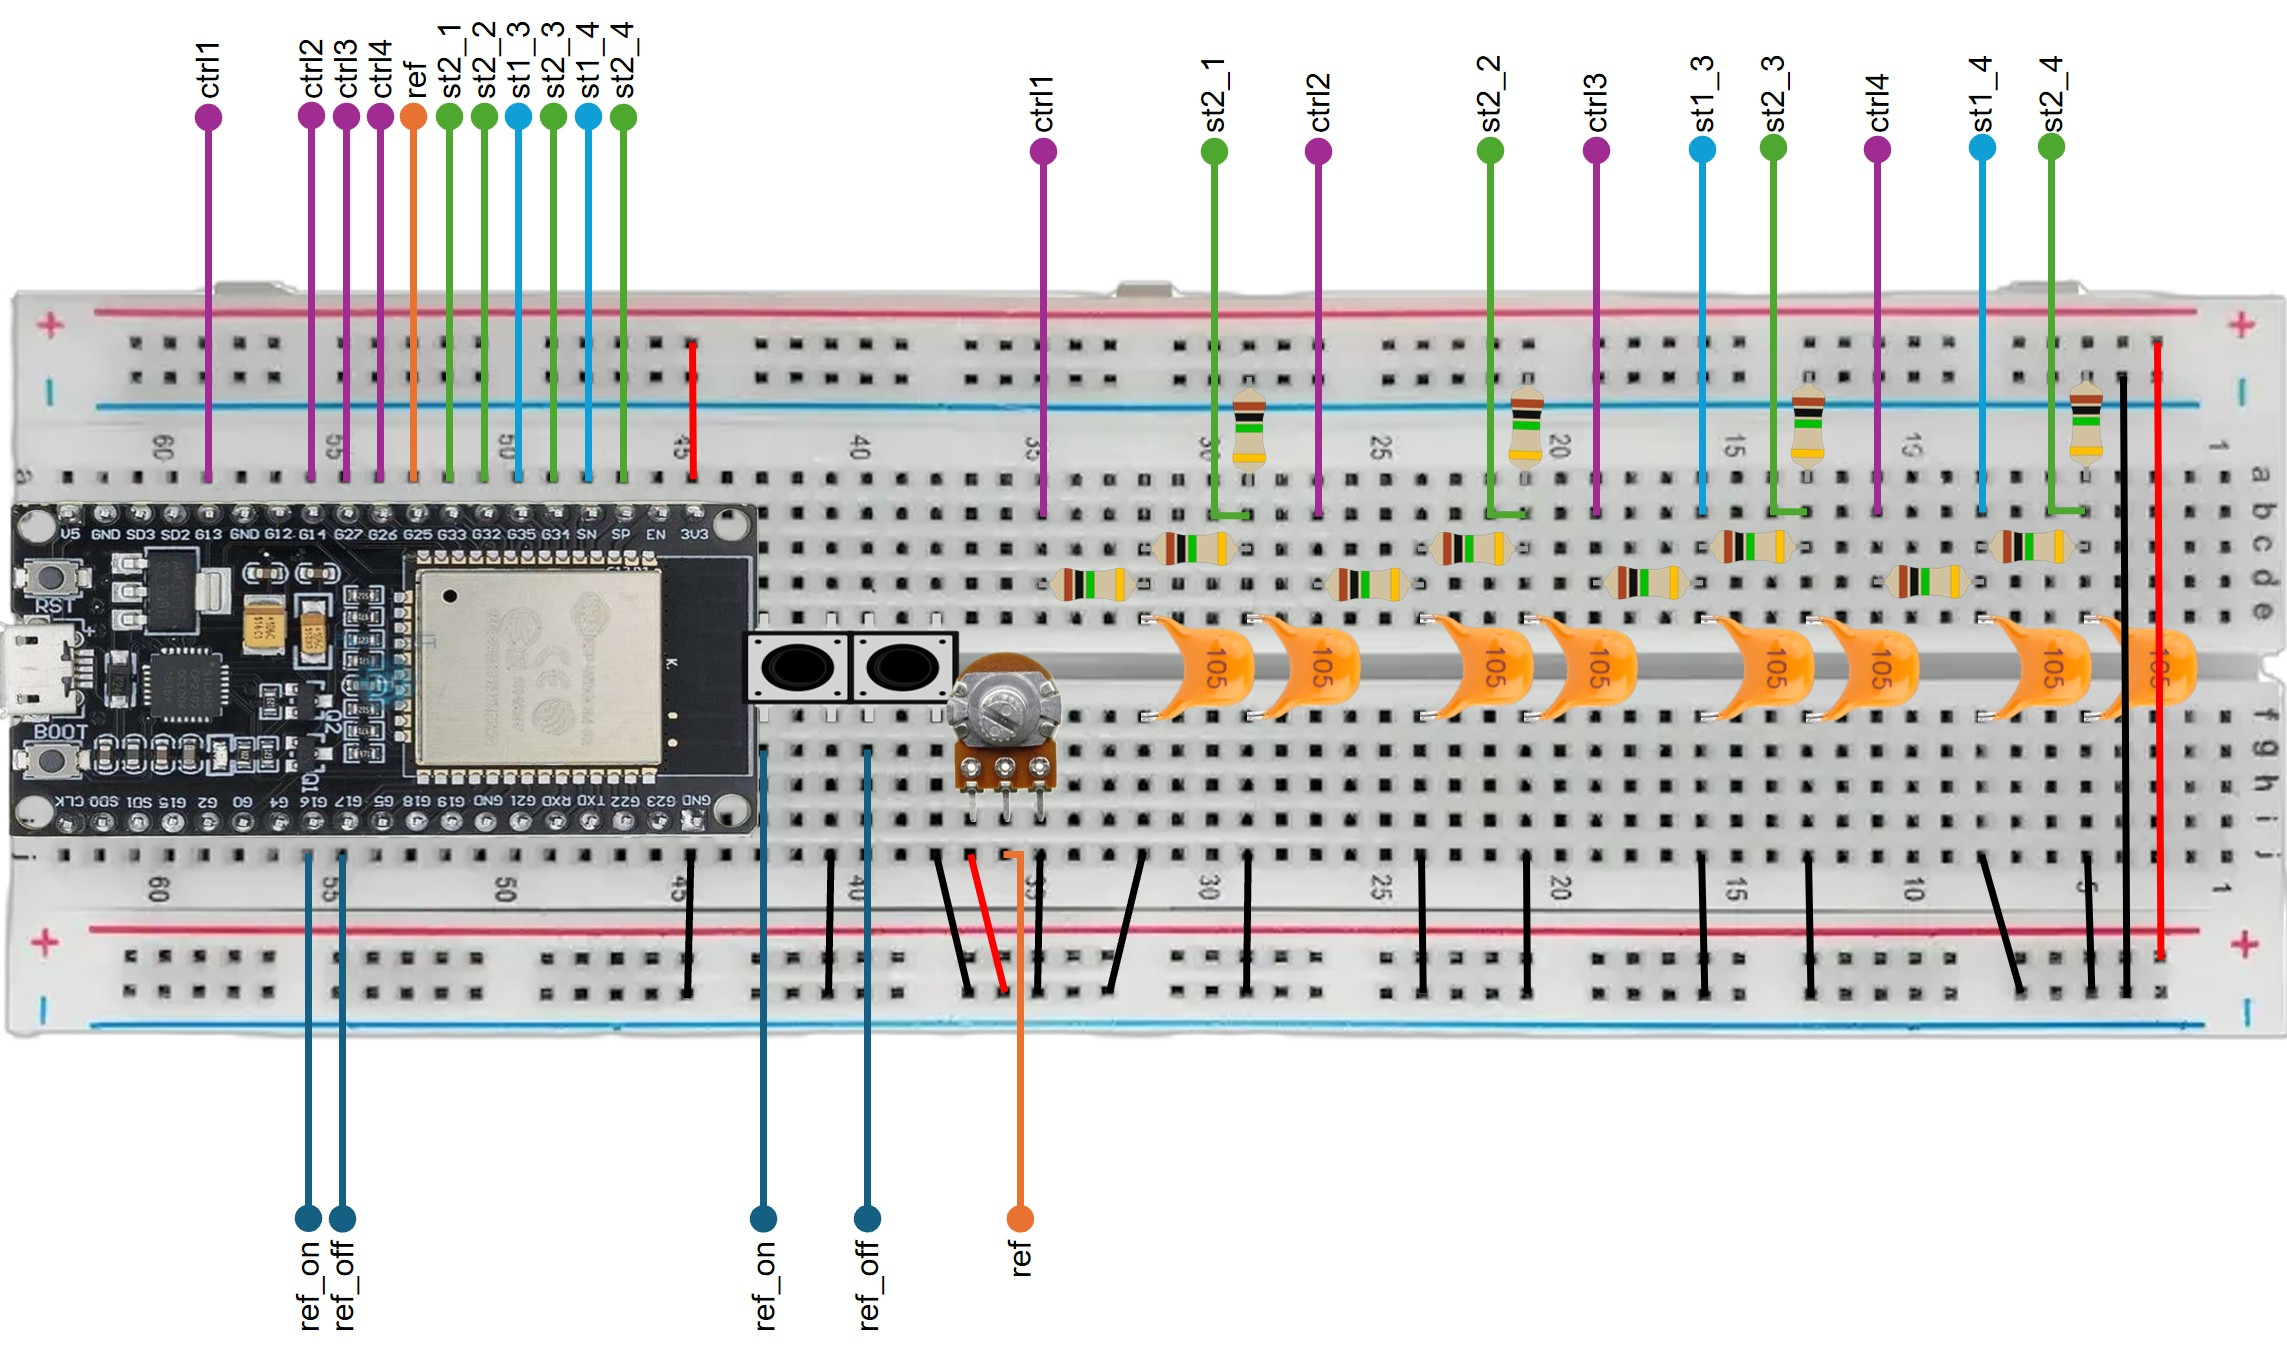
\includegraphics[width=0.9\textwidth]{Imagenes/proto_digital.jpg}
\caption{Diagrama general de conexiones del sistema implementado en protoboard.}
\label{fig:proto_digital}
\end{figure}

Por otro lado, la implementación física final del sistema se muestra en la Figura \ref{fig:proto}, donde se observan las cuatro configuraciones RC construidas en paralelo sobre la tarjeta de pruebas.

\begin{figure}[H]
\centering
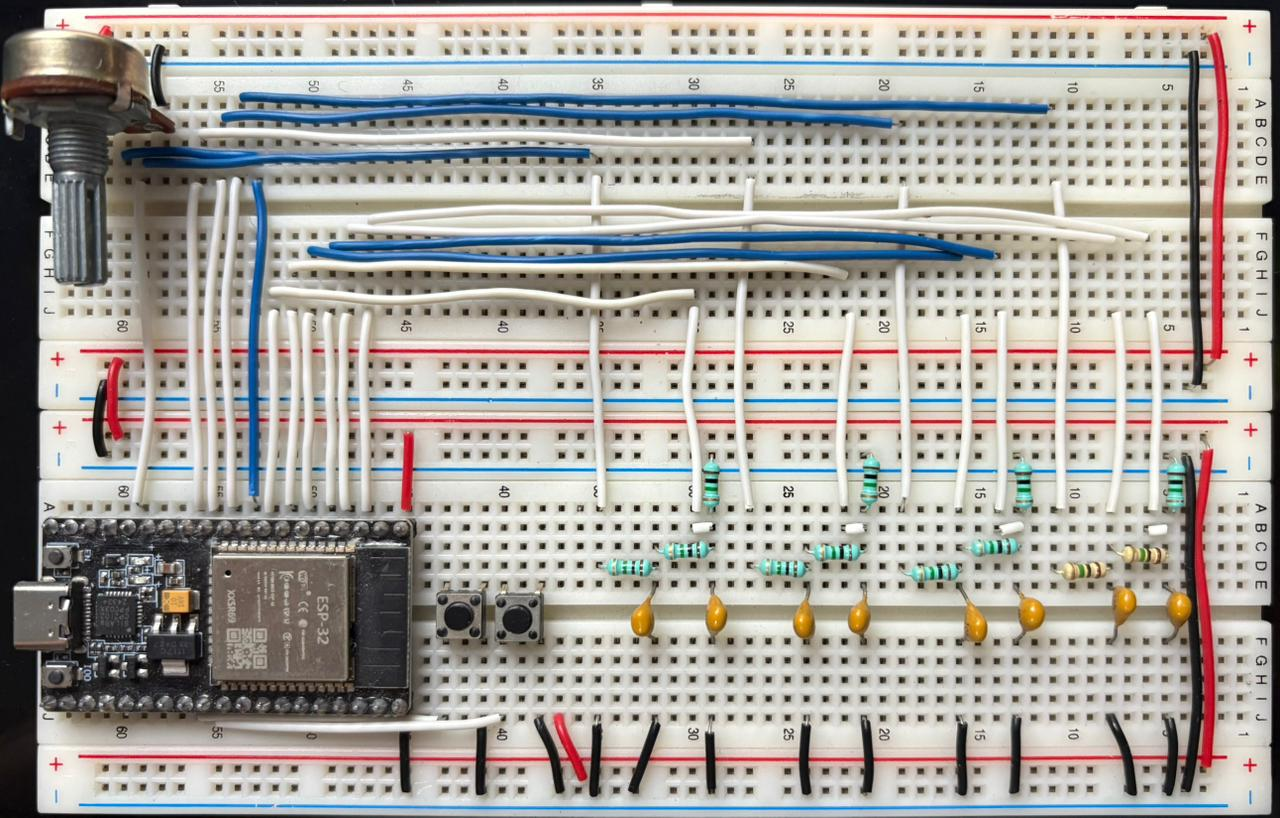
\includegraphics[width=\textwidth]{Imagenes/proto.jpeg}
\caption{Implementación física del sistema RC en protoboard.}
\label{fig:proto}
\end{figure}

La arquitectura implementada permite comparar simultáneamente distintas estrategias de control utilizando la misma referencia, el mismo tiempo de muestreo y condiciones físicas equivalentes. De esta manera, es posible evaluar el desempeño de cada controlador considerando variables como el seguimiento de referencia, el esfuerzo de control y la respuesta dinámica del sistema. Cada planta fue asociada a una estrategia de control distinta, permitiendo realizar la comparación experimental de manera simultánea y bajo condiciones equivalentes.

Adicionalmente, el ESP32 se encarga de realizar la adquisición de señales analógicas, el cálculo de las leyes de control en tiempo discreto y la generación de señales PWM aplicadas a cada una de las plantas implementadas.

%=========================================================
\section{Resultados experimentales y verificación de optimalidad}

Con el objetivo de verificar experimentalmente la optimalidad del controlador diseñado respecto al índice de desempeño definido en la Sección \ref{sec:performance}, se realizó la comparación entre el control óptimo LQR y tres estrategias de control adicionales: control por asignación de polos, control integral por asignación de polos y control con acción integral (LQI).

El controlador LQR se considera óptimo respecto al índice de desempeño planteado, debido a que su ganancia de retroalimentación se obtiene mediante la minimización explícita de dicha función de costo.

De manera similar, el controlador LQI también corresponde a una estrategia de control óptimo; sin embargo, su diseño se realiza sobre un sistema aumentado que incorpora un estado integral, por lo que minimiza una función de costo distinta asociada al sistema extendido.

Por otro lado, los controladores basados en asignación de polos no optimizan explícitamente una función de costo, sino que se diseñan a partir de especificaciones dinámicas deseadas.

Las mediciones fueron adquiridas mediante un sistema de monitoreo desarrollado en Python, el cual permite la visualización en tiempo real de las trayectorias de referencia, salida y señal de control de cada uno de los sistemas implementados. El sistema también almacena automáticamente los datos experimentales en archivos CSV para su posterior análisis.

\subsection{Adquisición de datos experimentales}

La adquisición de datos se realizó mediante comunicación serial entre el microcontrolador ESP32 y una interfaz desarrollada con \textit{PySide6}, mientras que la visualización se implementó utilizando \textit{PyQtGraph}. Este sistema permite la recepción de paquetes binarios que contienen las variables del sistema, los cuales son decodificados y almacenados en estructuras tipo cola para su visualización en tiempo real.

Al finalizar cada experimento, los datos son exportados a formato CSV mediante la librería \textit{pandas}, lo que permite su análisis numérico y la evaluación del desempeño de cada controlador.

\subsection{Resultados experimentales}

En la Figura \ref{fig:reporte_monitor} se muestra un ejemplo del reporte generado automáticamente por el sistema de monitoreo, donde se observan las respuestas de los cuatro controladores ante la misma referencia.

\begin{figure}[H]
\centering

\includegraphics[width=0.9\textwidth]{Imagenes/reporte_monitor.png}
\caption{Resultados experimentales obtenidos mediante el sistema de monitoreo en tiempo real.}
\label{fig:reporte_monitor}
\end{figure}

A partir de los datos obtenidos, se evaluó el índice de desempeño definido previamente. Este cálculo se realizó de forma numérica utilizando la aproximación discreta del criterio cuadrático, considerando las trayectorias de los estados y la señal de control registrada durante el experimento.

\subsection{Cálculo del índice de desempeño}

El índice de desempeño fue implementado directamente en el sistema de monitoreo, utilizando los datos almacenados en el archivo CSV generado al finalizar la adquisición.

El fragmento principal del código utilizado para este cálculo se muestra a continuación:

\begin{lstlisting}[language=Python, firstnumber=247, caption={Cálculo del índice de desempeño a partir de datos experimentales}, label={lst:indiceJ}]
def calcular_J(self, df):

    dt = df['t'].diff().fillna(0)

    resultados = []

    for i in range(1,5):
        x1 = df[f'X1_{i}']
        x2 = df[f'Y{i}']
        u  = df[f'U{i}']

        J = ((x1**2 + 5*x2**2 + u**2) * dt).sum()
        resultados.append(J)

    nombres = ["AdP","Int-AdP","LQR","LQI"]

    return resultados, nombres
\end{lstlisting}

Como se observa, el índice de desempeño se calcula de forma independiente para cada controlador, considerando la contribución de los estados y la energía de control.

\subsection{Comparación de controladores}

Los resultados obtenidos permiten comparar el desempeño de los cuatro esquemas de control bajo las mismas condiciones experimentales. El sistema de monitoreo genera automáticamente una comparación numérica del índice de desempeño \(J\), identificando el controlador con menor valor como el de mejor desempeño respecto al criterio planteado.

Como puede observarse en la Figura \ref{fig:reporte_monitor}, el controlador LQR presenta el menor valor de \(J\), lo cual resulta consistente con la teoría de control óptimo, ya que su ganancia fue obtenida mediante la minimización explícita del funcional definido en la Sección \ref{sec:performance}.

Por otro lado, aunque el controlador LQI también corresponde a una estrategia de control óptimo, este minimiza una función de costo distinta asociada al sistema aumentado con acción integral. Debido a ello, el desempeño obtenido respecto al índice original resulta inferior al obtenido mediante el LQR convencional.

Asimismo, los controladores basados en asignación de polos presentan valores mayores de \(J\), debido a que su diseño se basa en especificaciones dinámicas deseadas y no en la minimización explícita de una función de costo cuadrática.

\subsection{Discusión de resultados}

Los resultados experimentales validan que el controlador LQR presenta el mejor desempeño global respecto al índice de desempeño definido, obteniendo el menor valor de \(J\) entre todas las estrategias implementadas.

Aunque el controlador LQI incorpora acción integral y corresponde también a una estrategia de control óptimo, su diseño se realiza sobre un sistema aumentado y con una función de costo distinta, lo que produjo un incremento considerable en el valor del índice evaluado experimentalmente.

Por otro lado, los controladores diseñados mediante asignación de polos presentaron desempeños intermedios y mayores valores de esfuerzo de control, debido a que no consideran explícitamente un criterio de optimización durante su diseño.

En conjunto, los resultados experimentales confirman que la formulación del problema de control como una minimización explícita de un índice cuadrático permite obtener un mejor compromiso entre seguimiento de referencia y esfuerzo de control.

% =========================================================
\section{Conclusión}

En este trabajo se obtuvo el modelo matemático de un sistema eléctrico RC en forma de espacio de estados a partir del análisis del circuito mediante las leyes de Kirchhoff. Este modelo permitió describir la dinámica del sistema en función de los voltajes presentes en los capacitores y sirvió como base para el diseño de distintas estrategias de control.

Asimismo, se definió un índice de desempeño cuadrático que permitió formular el problema de control óptimo y diseñar un controlador LQR mediante la solución de la ecuación algebraica de Riccati. De manera complementaria, se desarrollaron estrategias adicionales de control mediante asignación de polos, control integral por asignación de polos y control óptimo con acción integral (LQI), con el propósito de comparar experimentalmente su desempeño.

Para las estrategias basadas en asignación de polos se implementó un observador de estados de orden completo, permitiendo estimar el estado no medido del sistema a partir de la salida disponible. Por otro lado, las implementaciones LQR y LQI emplearon medición directa de ambos estados.

Adicionalmente, se determinó una ganancia de prealimentación mediante cambio de coordenadas, permitiendo garantizar el seguimiento de referencias constantes sin error en estado estacionario para el controlador LQR.

Finalmente, se realizó la implementación experimental de cuatro plantas RC físicamente equivalentes utilizando un microcontrolador ESP32, lo que permitió ejecutar simultáneamente las distintas estrategias de control bajo las mismas condiciones experimentales. Los resultados obtenidos validan que el controlador LQR presenta el mejor desempeño respecto al índice de desempeño planteado, confirmando experimentalmente que la minimización explícita del funcional definido conduce a un mejor compromiso entre seguimiento de referencia y esfuerzo de control para el sistema considerado.

En conjunto, el trabajo integra el modelado físico del sistema, el diseño de controladores, la estimación de estados y la validación experimental, proporcionando una implementación completa de técnicas de control moderno aplicadas a un sistema dinámico real.

% =========================================================

\begin{thebibliography}{99}

\bibitem{Ogata}
K. Ogata,
\textit{Modern Control Engineering},
5th ed.
Upper Saddle River, NJ, USA:
Prentice Hall, 2010.

\bibitem{Kirk}
D. E. Kirk,
\textit{Optimal Control Theory: An Introduction},
Mineola, NY, USA:
Dover Publications, 2004.

\bibitem{Franklin}
G. F. Franklin, J. D. Powell, and A. Emami-Naeini,
\textit{Feedback Control of Dynamic Systems},
7th ed.
Boston, MA, USA:
Pearson, 2015.

\end{thebibliography}

% =========================================================
\newpage
\appendix

\section*{Apéndices}
\addcontentsline{toc}{section}{Apéndices}

\section{Códigos}

\subsection{Resolución numérica del controlador LQR}
\label{sec:SolveLQR}

\begin{lstlisting}[language=Python]
import numpy as np
from scipy.linalg import solve_continuous_are
from scipy.integrate import solve_ivp
import matplotlib.pyplot as plt

R1 = 1000
R2 = 1000
R3 = 1000
C1 = 1e-6
C2 = 1e-6

# matrices del sistema
A = np.array([[-1/(R1*C1)-1/(R2*C1), 1/(R2*C1)],
            [1/(R2*C2), -1/(R2*C2)-1/(R3*C2)]])

B = np.array([[1/(R1*C1)],
            [0]])

Q = np.array([[1, 0],
            [0, 5]])

R = np.array([[1]])

# resolver Riccati
P = solve_continuous_are(A,B,Q,R)

print("P =", P)

# ganancia LQR
K = np.linalg.inv(R) @ B.T @ P
print("K =", K)
\end{lstlisting}

\subsection{Análisis simbólico de la ecuación de Riccati}

\begin{lstlisting}[language=Python]
import numpy as np
from scipy.linalg import solve_continuous_are
from sympy import symbols, Matrix, solve, pprint

R1, C1, R2, C2, R3 = symbols('R1 C1 R2 C2 R3')

A = Matrix([[-1/(R1*C1)-1/(R2*C1), 1/(R2*C1)],
            [1/(R2*C2), -1/(R2*C2)-1/(R3*C2)]])

B = Matrix([[1/(R1*C1)],
            [0]])
            
Q = Matrix([[1, 0],
              [0, 5]])
              
R = Matrix([1])

p11, p12, p22 = symbols('p11 p12 p22')

P = Matrix([[p11, p12],
            [p12, p22]])

Rinv = R.inv()

riccati = A.T*P + P*A - P*B*Rinv*B.T*P + Q

pprint(riccati)
\end{lstlisting}

\subsection{Resolución numérica del controlador LQI}
\label{sec:SolveLQI}

El controlador LQI fue desarrollado mediante el aumento del sistema con acción integral y la posterior solución de la ecuación algebraica de Riccati, siguiendo el enfoque presentado en \cite{Kirk}.

\begin{lstlisting}[language=Python]
#Control LQI
import numpy as np
from scipy.linalg import solve_continuous_are
from scipy.integrate import solve_ivp
import matplotlib.pyplot as plt

R1 = 1000
R2 = 1000
R3 = 1000
C1 = 1e-6
C2 = 1e-6

# matrices del sistema
A = np.array([[-1/(R1*C1)-1/(R2*C2), 1/(R2*C1)],
            [1/(R2*C2), -1/(R2*C2)-1/(R3*C2)]])

B = np.array([[1/(R1*C1)],
            [0]])

C = np.array([[0, 1]])

# sistema aumentado (LQI)

Aa = np.block([
    [np.zeros((1,1)), -C],
    [np.zeros((2,1)),  A]
])

Ba = np.vstack([
    np.zeros((1,1)),
    B
])

print("Aa =\n", Aa)
print("Ba =\n", Ba)

Qa = np.diag([10, 1, 5])

print("Qa =\n", Qa)

R = np.array([[1]])

# resolver Riccati
P = solve_continuous_are(Aa,Ba,Qa,R)

print("P =", P)

# ganancia LQI
K = np.linalg.inv(R) @ Ba.T @ P
print("K =", K)
\end{lstlisting}

\subsection{Implementación en microcontrolador (ESP32)}
\label{sec:esp32}

\begin{lstlisting}[language=C++]
// ================= PINES =================
#define X2_1 33
#define X2_2 32
#define X1_3 35
#define X2_3 34
#define X1_4 39
#define X2_4 36

#define REF_PIN 25

#define PWM1 13
#define PWM2 14
#define PWM3 27
#define PWM4 26

#define BTN_ON 16
#define BTN_OFF 17

// ================= PWM =================
#define PWM_FREQ 5000
#define PWM_RES 8

// ================= PLANTA =================
#define R1 1000000
#define R2 1000000
#define R3 1000000
#define C1 0.000001
#define C2 0.000001

#define mX (3.3/4095.0)
#define mU (255.0/3.3)

// ================= TIEMPO =================
unsigned long TS = 50;
float Tseg = 0.05;
unsigned long TIC = 0, TS_code = 0, TC = 0;

// ================= VARIABLES =================
float R = 0;
bool Habilitado = 0;

// ===== MODELO =====
float Am11, Am12, Am21, Am22, Bm1, Bm2;

// ================= SISTEMA 1 (POLOS) =================
float Xe1_1=0, Xe2_1=0;
float K1_1, K2_1, Kp_1;
float H1_1, H2_1;
float U1=0, Y1=0;

// ================= SISTEMA 2 (INTEGRAL POLOS) =================
float Xe1_2=0, Xe2_2=0, X0_2=0;
float K0_2, K1_2, K2_2;
float H1_2, H2_2;
float U2=0, Y2=0;

// ================= SISTEMA 3 (LQR) =================
float K1_3=0.41421356;
float K2_3=0.41421356;
float Kp_3;
float X13=0, X23=0;
float U3=0, Y3=0;

// ================= SISTEMA 4 (LQI) =================
float K0_4=3.16227766;
float K1_4=0.41495869;
float K2_4=0.41601274;
float X0_4=0;
float X14=0, X24=0;
float U4=0, Y4=0;

// =========================================================
// ======================= SETUP ============================
// =========================================================
void setup(){
  Serial.begin(115200);

  pinMode(BTN_ON, INPUT_PULLUP);
  pinMode(BTN_OFF, INPUT_PULLUP);

  // PWM
  ledcSetup(0, PWM_FREQ, PWM_RES);
  ledcSetup(1, PWM_FREQ, PWM_RES);
  ledcSetup(2, PWM_FREQ, PWM_RES);
  ledcSetup(3, PWM_FREQ, PWM_RES);

  ledcAttachPin(PWM1,0);
  ledcAttachPin(PWM2,1);
  ledcAttachPin(PWM3,2);
  ledcAttachPin(PWM4,3);

  // ===== MODELO =====
  float p11 = R1*C1;
  float p12 = R1*C2;
  float p21 = R2*C1;
  float p22 = R2*C2;
  float p32 = R3*C2;

  Am11 = -1/p11 - 1/p21;
  Am12 = 1/p21;
  Am21 = 1/p22;
  Am22 = -1/p22 - 1/p32;
  Bm1 = 1/p11;
  Bm2 = 0;

  // =====================================================
  // SISTEMA 1 (ASIGNACIÓN DE POLOS)
  // =====================================================
  float a1r=-1.25, a1i=-1.7320508;   //polos controlador
  float a2r=-1.25, a2i=1.7320508;
  float b1r=-10, b2r=-10;            //polos observador

  float sum_a = -(a1r + a2r);
  float prod_a = a1r*a2r - a1i*a2i;
  float sum_b = -(b1r + b2r);
  float prod_b = b1r*b2r;


  //Ganancias de controlador
  K1_1 = p11*(sum_a - 1/p11 - 1/p21 - 1/p22 - 1/p32);
  K2_1 = p12*p22*(prod_a - 1/(p11*p22) - 1/(p11*p32) - 1/(p21*p22) - 1/(p21*p32)
          - K1_1/(p11*p22) - K1_1/(p11*p32) + 1/(p21*p22));
  Kp_1 = K1_1 + K2_1 + 1 + (K1_1*R2+R1+R2)/R3;  //Ganancia de seguimiento mediante cambio de coordenadas


  //Observador de Luenberger
  H2_1 = sum_b - 1/p11 - 1/p21 - 1/p22 - 1/p32;
  H1_1 = p22*(prod_b - 1/(p11*p22) -1/(p11*p32) - 1/(p21*p22)
          - 1/(p21*p32) - H2_1/p11 - H2_1/p21 + 1/(p21*p22));

  // =====================================================
  // SISTEMA 2 (INTEGRAL)
  // =====================================================
  float a3r=-1;  //polo integral

  float sum_ai = -(a1r + a2r + a3r);
  float prod_ai = -(a1r*a2r - a1i*a2i)*a3r;

  //Ganancias de controlador
  K0_2 = p11*p22*prod_ai;
  K1_2 = p11*(sum_ai - 1/p11 - 1/p21 - 1/p22 - 1/p32);
  K2_2 = p11*(p22*(a1r*a3r + a2r*a3r + a1r*a2r)
          - 1/(p21*p32) - (1+K1_2)/(p11*p32)) - 1 - K1_2;

  //Mismo observador de Luenberger
  H2_2 = H2_1;
  H1_2 = H1_1;

  // =====================================================
  // SISTEMA 3 (LQR)
  // =====================================================
  Kp_3 = K1_3 + K2_3 + 1 + (K1_3*R2+R1+R2)/R3;  //Ganancia de seguimiento mediante cambio de coordenadas

}

// =========================================================
// ======================== LOOP ============================
// =========================================================
void loop(){

  if(digitalRead(BTN_ON) == LOW) Habilitado=1;
  else if(digitalRead(BTN_OFF) == LOW) Habilitado=0;

  R = Habilitado*(analogRead(REF_PIN)*mX);  //Referencia

  control_1();
  control_2();
  control_3();
  control_4();

  // ===== PWM =====
  ledcWrite(0, U1*mU);
  ledcWrite(1, U2*mU);
  ledcWrite(2, U3*mU);
  ledcWrite(3, U4*mU);

  // coms_arduino_ide();

  coms_python(&R,
              &Xe1_1,&Y1,&U1,  //sistema 1
              &Xe1_2,&Y2,&U2,  //sistema 2
              &X13,&Y3,&U3,    //sistema 3
              &X14,&Y4,&U4);   //sistema 4

  espera();
}

// ===== Control por Asignación de polos =====
void control_1(){
  Y1 = analogRead(X2_1)*mX;  //estado 2 y salida
  float e1 = Y1 - Xe2_1;

  float f1_1 = Am11*Xe1_1 + Am12*Xe2_1 + Bm1*U1 + H1_1*e1;  //Dinamica estado 1 observador
  float f2_1 = Am21*Xe1_1 + Am22*Xe2_1 + H2_1*e1;           //Dinamica estado 2 observador

  Xe1_1 += Tseg*f1_1;  //Integrador estado 1 mediante Euler
  Xe2_1 += Tseg*f2_1;  //Integrador estado 2 mediante Euler
  
  //Ley de control u = -Kx
  U1 = Kp_1*R - K1_1*Xe1_1 - K2_1*Xe2_1;
  
  U1 = constrain(U1,0,3.3);  //saturacion
}

// ===== Control Integral por Asignación de polos =====
void control_2(){
  Y2 = analogRead(X2_2)*mX;  //estado 2 y salida

  //observador
  float e2 = Y2 - Xe2_2;

  float f1_2 = Am11*Xe1_2 + Am12*Xe2_2 + Bm1*U2 + H1_2*e2;  //Dinámica estado 1 observador
  float f2_2 = Am21*Xe1_2 + Am22*Xe2_2 + H2_2*e2;           //Dinámica estado 2 observador

  Xe1_2 += Tseg*f1_2;      //Integrador estado 1 mediante Euler
  Xe2_2 += Tseg*f2_2;      //Integrador estado 2 mediante Euler
  X0_2 += Tseg*(R - Y2);  //estado 0
  
  //Ley de control u = -Kx
  U2 = K0_2*X0_2 - K1_2*Xe1_2 - K2_2*Xe2_2;
  
  U2 = constrain(U2,0,3.3);  //saturación
}

// ===== Control LQR =====
void control_3(){
  X13 = analogRead(X1_3)*mX;  //estado 1
  X23 = analogRead(X2_3)*mX;  //estado 2
  Y3 = X23;  //salida
  //Ley de control u = -Kx
  U3 = Kp_3*R - K1_3*X13 - K2_3*X23;

  U3 = constrain(U3,0,3.3);  //saturación
}

// ===== Control LQI =====
void control_4(){
  X14 = analogRead(X1_4)*mX;  //estado 1
  X24 = analogRead(X2_4)*mX;  //estado 2
  Y4 = X24;  //salida

  X0_4 += Tseg*(R - Y4);  //estado 0
  
  //Ley de control u = -Kx
  U4 = K0_4*X0_4 - K1_4*X14 - K2_4*X24;

  U4 = constrain(U4,0,3.3);  //saturación
}

//Muestreo uniforme
void espera(){   
  TS_code = millis()- TIC;
  TC = TS - TS_code;
  if (TS_code < TS) delay(TC);
  TIC = millis();
}

//Comunicación con serial monitor y serial plotter
void coms_arduino_ide(){

    Serial.print("R:"); Serial.print(R);  //referencia

    Serial.print(" | Y1:"); Serial.print(Y1); Serial.print(" U1:"); Serial.print(U1);  //sistema 1
    Serial.print(" | Y2:"); Serial.print(Y2); Serial.print(" U2:"); Serial.print(U2);     //sistema 2
    Serial.print(" | Y3:"); Serial.print(Y3); Serial.print(" U3:"); Serial.print(U3);     //sistema 3
    Serial.print(" | Y4:"); Serial.print(Y4); Serial.print(" U4:"); Serial.println(U4);   //sistema 4
}

//Comunicación con monitor de pyhton
void coms_python(float* Rp,
                 float* X11,float* Y1p, float* U1p,
                 float* X12,float* Y2p, float* U2p,
                 float* X13,float* Y3p, float* U3p,
                 float* X14,float* Y4p, float* U4p)
{
  float t = TIC/1000.0;

  byte* tB  = (byte*)(&t);  //tiempo
  byte* RB  = (byte*)(Rp);  //referencia

  byte* X1B1 = (byte*)(X11);  //estado 1 sistema 1 AdP
  byte* Y1B  = (byte*)(Y1p);  //salida sistema 1 AdP
  byte* U1B  = (byte*)(U1p);  //control sistema 1 AdP

  byte* X1B2 = (byte*)(X12);  //estado 1 sistema 2 Integral AdP
  byte* Y2B  = (byte*)(Y2p);  //salida sistema 2 Integral AdP
  byte* U2B  = (byte*)(U2p);  //control sistema 2 Integral AdP

  byte* X1B3 = (byte*)(X13);  //estado 1 sistema 3 LQR
  byte* Y3B  = (byte*)(Y3p);  //salida sistema 3 LQR
  byte* U3B  = (byte*)(U3p);  //control sistema 3 LQR

  byte* X1B4 = (byte*)(X14);  //estado 1 sistema 4 LQR
  byte* Y4B  = (byte*)(Y4p);  //salida sistema 4 LQR
  byte* U4B  = (byte*)(U4p);  //control sistema 4 LQR

  byte buf[56] = {
    tB[0],tB[1],tB[2],tB[3],  //tiempo
    RB[0],RB[1],RB[2],RB[3],  //Referencia

    X1B1[0],X1B1[1],X1B1[2],X1B1[3],  //estado 1 sistema 1 AdP
    Y1B[0],Y1B[1],Y1B[2],Y1B[3],      //salida sistema 1 AdP
    U1B[0],U1B[1],U1B[2],U1B[3],      //control sistema 1 AdP

    X1B2[0],X1B2[1],X1B2[2],X1B2[3],  //estado 1 sistema 2 Integral AdP
    Y2B[0],Y2B[1],Y2B[2],Y2B[3],      //salida sistema 2 Integral AdP
    U2B[0],U2B[1],U2B[2],U2B[3],      //control sistema 2 Integral AdP

    X1B3[0],X1B3[1],X1B3[2],X1B3[3],  //estado 1 sistema 3 LQR
    Y3B[0],Y3B[1],Y3B[2],Y3B[3],      //salida sistema 3 LQR
    U3B[0],U3B[1],U3B[2],U3B[3],      //control sistema 3 LQR

    X1B4[0],X1B4[1],X1B4[2],X1B4[3],  //estado 1 sistema 4 LQR
    Y4B[0],Y4B[1],Y4B[2],Y4B[3],      //salida sistema 4 LQR
    U4B[0],U4B[1],U4B[2],U4B[3]       //control sistema 4 LQR
  };

  uint8_t header[2] = {0xAA, 0x55};
  Serial.write(header, 2);
  Serial.write(buf, 56);
}
\end{lstlisting}

\subsection{Monitor de adquisición y evaluación experimental}
\label{sec:monitor}

\begin{lstlisting}[language=Python]
#!/usr/bin/env python

import sys
import datetime
import os
from threading import Thread
import serial
import time
import collections
import struct
import copy
import pandas as pd
import matplotlib.pyplot as plt
import platform
import subprocess

from PySide6.QtWidgets import (
    QApplication,
    QMainWindow,
    QWidget,
    QGridLayout,
    QLabel,
    QPushButton,
    QLineEdit,
    QVBoxLayout,
    QHBoxLayout,
    QCheckBox,
    QMessageBox
)
from PySide6.QtCore import QTimer, Qt
import pyqtgraph as pg

# ================= CONFIG =================
def load_config():

    if getattr(sys, 'frozen', False):
        base_dir = os.path.dirname(sys.executable)
    else:
        base_dir = os.path.dirname(os.path.abspath(__file__))
    
    config_dir = os.path.join(base_dir, "config")
    config_path = os.path.join(config_dir, "config.ini")

    if not os.path.exists(config_path):
        return None

    try:
        df = pd.read_csv(config_path)

        config = {
            "port": df["port"][0],
            "baud": int(df["baud"][0]),
            "plotLength": int(df["plotLength"][0]),
            "interval": int(df["interval"][0]),
            "ymin": float(df["ymin"][0]),
            "ymax": float(df["ymax"][0]),
            "saveCSV": str(df["saveCSV"][0]).lower() in ["1", "true", "yes"]
        }

        QMessageBox.information(
            None,
            "Configuración",
            "Configuración cargada desde config.ini"
        )

        return config

    except Exception as e:

        QMessageBox.critical(
            None,
            "Error",
            f"Error leyendo config.ini:\n\n{e}"
        )

        return None

def save_config(port, baud, plotLength, interval, ymin, ymax, saveCSV):

    if getattr(sys, 'frozen', False):
        base_dir = os.path.dirname(sys.executable)
    else:
        base_dir = os.path.dirname(os.path.abspath(__file__))
    
    config_dir = os.path.join(base_dir, "config")
    os.makedirs(config_dir, exist_ok=True)
    
    config_path = os.path.join(config_dir, "config.ini")

    df = pd.DataFrame([{
        "port": port,
        "baud": baud,
        "plotLength": plotLength,
        "interval": interval,
        "ymin": ymin,
        "ymax": ymax,
        "saveCSV": saveCSV
    }])

    df.to_csv(config_path, index=False)

    QMessageBox.information(
        None,
        "Configuración guardada",
        f"Configuración guardada en:\n\n{config_path}"
    )

def clear(): 
    if os.name == "posix":
        os.system ("clear")
    elif os.name in ("ce", "nt", "dos"):
        os.system ("cls")

# ================= SERIAL =================
class serialPlot:
    def __init__(self, port, baud, plotLength):

        self.plotMaxLength = plotLength

        self.rawData = bytearray(56)  # NUEVO

        self.buffer = bytearray()

        # [R,X1,Y,U] x 4 = 16 buffers
        self.data = [collections.deque([0]*plotLength, maxlen=plotLength) for _ in range(16)]

        self.packetQueue = collections.deque()
        self.csvPackets = []

        self.isRun = True
        self.thread = None

        self.serialConnection = serial.Serial(port, baud, timeout=4)

    def readSerialStart(self):
        self.thread = Thread(target=self.backgroundThread)
        self.thread.daemon = True
        self.thread.start()

    def backgroundThread(self):
        time.sleep(1)
        self.serialConnection.reset_input_buffer()
    
        while self.isRun:

            try:
        
                data = self.serialConnection.read(
                    self.serialConnection.in_waiting or 1
                )
        
                if data:
                    self.buffer.extend(data)
        
            except serial.SerialException as e:
        
                print("\nError serial:")
                print(e)
        
                self.isRun = False
                break
    
            #sincronización de paquetes
            while True:
                start = self.buffer.find(b'\xAA\x55')
    
                if start == -1:
                    self.buffer = self.buffer[-2:]
                    break
    
                if len(self.buffer) < start + 2 + 56:
                    break  # esperar más datos
    
                packet = self.buffer[start+2:start+2+56]
                self.buffer = self.buffer[start+2+56:]
    
                self.packetQueue.append(packet)
                self.csvPackets.append(packet)
            
    def close(self, saveCSV):
        self.isRun = False
        if self.thread is not None:
            self.thread.join(timeout=1)
        
        if self.serialConnection.is_open:
            self.serialConnection.close()

        if saveCSV:
            self.saveCSV()

    def saveCSV(self):

        if not self.csvPackets:
        
            QMessageBox.warning(
                None,
                "Sin datos",
                "No hay datos para guardar."
            )
        
            return
            
        data = []

        for packet in self.csvPackets:
            values = []
            for i in range(14):
                value, = struct.unpack('f', packet[i*4:(i+1)*4])
                values.append(value)

            data.append(values)

        df = pd.DataFrame(data, columns=[
            't','R',
            'X1_1','Y1','U1',
            'X1_2','Y2','U2',
            'X1_3','Y3','U3',
            'X1_4','Y4','U4'
        ])

        # Ruta base compatible con .py y .exe
        if getattr(sys, 'frozen', False):
            base_dir = os.path.dirname(sys.executable)
        else:
            base_dir = os.path.dirname(os.path.abspath(__file__))
        
        # Carpeta /data
        data_dir = os.path.join(base_dir, "data")
        os.makedirs(data_dir, exist_ok=True)
        
        filename = datetime.datetime.now().strftime("%Y%m%d_%H%M%S")
        
        # Ruta completa del CSV
        path = os.path.join(data_dir, f"datos_{filename}.csv")

        df.to_csv(path, index=False)

        QMessageBox.information(
            None,
            "CSV guardado",
            f"CSV guardado en:\n\n{path}"
        )

        resultados, nombres = self.calcular_J(df)
        self.generar_reporte(df, resultados, nombres, filename, path)

    def calcular_J(self, df):

        dt = df['t'].diff().fillna(0)
    
        resultados = []
    
        for i in range(1,5):
            x1 = df[f'X1_{i}']
            x2 = df[f'Y{i}']
            u  = df[f'U{i}']
    
            J = ((x1**2 + 5*x2**2 + u**2) * dt).sum()
            resultados.append(J)
    
        nombres = ["AdP","Int-AdP","LQR","LQI"]
    
        return resultados, nombres

    def generar_reporte(self, df, resultados, nombres, filename, path):

        t = df['t']
        R = df['R']
    
        fig, axs = plt.subplots(2, 2, figsize=(12, 8))
        axs = axs.flatten()
    
        for i in range(4):
            ax = axs[i]
        
            Y = df[f'Y{i+1}']
            U = df[f'U{i+1}']
        
            ax.plot(t, R, 'r', label='Referencia')
            ax.plot(t, Y, 'k', label='Salida')
            ax.plot(t, U, 'b--', label='Control')
        
            ax.set_title(nombres[i])
            ax.grid()
        
            if i == 0:
                ax.legend()
    
        # Mejor índice
        best = resultados.index(min(resultados))
        
        # Título general
        fig.suptitle(filename, fontsize=14)
        
        # === NUEVO BLOQUE DE TEXTO ===
        
        # Título del índice
        fig.text(0.5, 0.14, "Índice de desempeño", ha='center', fontsize=12, weight='bold')
        
        # Fórmula (LaTeX)
        fig.text(0.5, 0.11, r"$J = \int (x^T Q x + u^T R u)\, dt$", ha='center', fontsize=11)
        
        # Nombres y valores alineados por columnas
        for i in range(4):
            fig.text(0.2 + i*0.2, 0.08, nombres[i], ha='center', fontsize=10)
            fig.text(0.2 + i*0.2, 0.05, f"J = {resultados[i]:.2f}", ha='center', fontsize=10)
        
        # Mejor controlador
        mejor_texto = f"MEJOR: {nombres[best]}"
        fig.text(0.5, 0.02, mejor_texto, ha='center', fontsize=12, weight='bold')
    
        plt.tight_layout(rect=[0, 0.16, 1, 0.95])
    
        # Guardar imagen
        img_path = path.replace(".csv", ".png")
        plt.savefig(img_path, dpi=300)
        
        manager = plt.get_current_fig_manager()

        try:
            manager.window.showMaximized()
        except:
            pass
        
        plt.show(block=False)
        plt.pause(0.1)
        
        QMessageBox.information(
            None,
            "Reporte generado",
            f"Imagen guardada en:\n\n{img_path}"
        )

# ================= SETUP WINDOW =================
class SetupWindow(QWidget):

    def __init__(self):
        super().__init__()

        self.setWindowTitle("Monitor Serial v2.0 - FIME UANL")
        self.setMinimumWidth(350)

        layout = QVBoxLayout()

        title = QLabel(
            "Monitor de Puerto Serial\n"
            "v2.0 - 7 de mayo del 2026\n"
            "Departamento de Electrónica y Automatización\n"
            "FIME - UANL"
        )

        title.setStyleSheet("""
            font-size: 14pt;
            font-weight: bold;
        """)
        
        title.setAlignment(Qt.AlignCenter)
        
        layout.addWidget(title)

        # ===== Inputs =====

        self.portEdit = QLineEdit("COM4")
        self.baudEdit = QLineEdit("115200")
        self.samplesEdit = QLineEdit("50")
        self.intervalEdit = QLineEdit("50")
        self.yminEdit = QLineEdit("-0.1")
        self.ymaxEdit = QLineEdit("3.3")

        layout.addWidget(QLabel("Puerto"))
        layout.addWidget(self.portEdit)

        layout.addWidget(QLabel("Baudrate"))
        layout.addWidget(self.baudEdit)

        layout.addWidget(QLabel("Samples"))
        layout.addWidget(self.samplesEdit)

        layout.addWidget(QLabel("Intervalo (ms)"))
        layout.addWidget(self.intervalEdit)

        layout.addWidget(QLabel("Y min"))
        layout.addWidget(self.yminEdit)

        layout.addWidget(QLabel("Y max"))
        layout.addWidget(self.ymaxEdit)

        # ===== Checkboxes =====

        self.saveCSVCheck = QCheckBox("Guardar CSV")
        self.saveConfigCheck = QCheckBox("Guardar configuración")
        self.useConfigCheck = QCheckBox("Usar configuración guardada")

        layout.addWidget(self.saveCSVCheck)
        layout.addWidget(self.saveConfigCheck)
        layout.addWidget(self.useConfigCheck)

        # ===== Botón =====

        self.startButton = QPushButton("INICIAR")
        self.startButton.clicked.connect(self.startMonitor)

        layout.addWidget(self.startButton)

        self.setLayout(layout)

        # ===== Cargar config automáticamente =====

        self.config = load_config()

        if self.config:
            self.useConfigCheck.setChecked(True)
            self.saveCSVCheck.setChecked(self.config["saveCSV"])
            self.portEdit.setText(str(self.config["port"]))
            self.baudEdit.setText(str(self.config["baud"]))
            self.samplesEdit.setText(str(self.config["plotLength"]))
            self.intervalEdit.setText(str(self.config["interval"]))
            self.yminEdit.setText(str(self.config["ymin"]))
            self.ymaxEdit.setText(str(self.config["ymax"]))

    def startMonitor(self):

        try:

            # ===== Config guardada =====

            if self.useConfigCheck.isChecked() and self.config:

                port = self.config["port"]
                baud = self.config["baud"]
                plotLength = self.config["plotLength"]
                interval = self.config["interval"]
                ymin = self.config["ymin"]
                ymax = self.config["ymax"]

            else:

                port = self.portEdit.text()
                baud = int(self.baudEdit.text())
                plotLength = int(self.samplesEdit.text())
                interval = int(self.intervalEdit.text())
                ymin = float(self.yminEdit.text())
                ymax = float(self.ymaxEdit.text())

            saveCSV = self.saveCSVCheck.isChecked()

            # ===== Guardar config =====

            if self.saveConfigCheck.isChecked():

                save_config(
                    port,
                    baud,
                    plotLength,
                    interval,
                    ymin,
                    ymax,
                    saveCSV
                )

            # ===== Serial =====

            self.serialObj = serialPlot(
                port,
                baud,
                plotLength
            )

            self.serialObj.readSerialStart()

            # ===== Monitor =====

            self.monitor = Monitor(
                self.serialObj,
                interval,
                ymin,
                ymax,
                saveCSV
            )

            self.monitor.showMaximized()

            self.hide()

            # guardar para closeEvent
            self.saveCSV = saveCSV

        except Exception as e:

            QMessageBox.critical(
                self,
                "Error",
                str(e)
            )

# ================= GUI =================
class Monitor(QMainWindow):      
    def __init__(self, serialObj, interval, ymin, ymax, saveCSV):
        
        super().__init__()

        self.setWindowTitle("Monitor de Control")

        self.s = serialObj

        central = QWidget()
        self.setCentralWidget(central)

        layout = QGridLayout()
        central.setLayout(layout)

        self.plots = []
        self.curves = []

        self.names = ["Control por Asignación de Polos", "Control Integral por Asignación de Polos", "Control LQR", "Control LQI"]
        for i in range(4):
            p = pg.PlotWidget(title=self.names[i])
            p.setYRange(ymin, ymax)
            p.setBackground('w')
            p.showGrid(x=True, y=True)
            p.addLegend()

            r = p.plot(
                pen=pg.mkPen('r', width=2),
                name='Referencia'
            )
            
            y = p.plot(
                pen=pg.mkPen('k', width=2),
                name='Salida'
            )
            
            u = p.plot(
                pen=pg.mkPen(color='b', width=2, style=Qt.DashLine),
                name='Control'
            )

            self.plots.append(p)
            self.curves.append((r,y,u))

            layout.addWidget(p, i//2, i%2)

        self.timer = QTimer()
        self.timer.timeout.connect(self.update)
        self.timer.start(interval)
        self.saveCSV = saveCSV

    def update(self):

        if len(self.s.packetQueue) == 0:
            return

        packet = self.s.packetQueue[-1]
        self.s.packetQueue.clear()

        values = [struct.unpack('f', packet[i*4:(i+1)*4])[0] for i in range(14)]

        R = values[1]

        idx = 2

        for i in range(4):
            X1 = values[idx]
            Y  = values[idx+1]
            U  = values[idx+2]
            idx += 3

            self.s.data[i*4].append(R)
            self.s.data[i*4+1].append(X1)
            self.s.data[i*4+2].append(Y)
            self.s.data[i*4+3].append(U)

            r,y,u = self.curves[i]

            r.setData(list(self.s.data[i*4]))
            y.setData(list(self.s.data[i*4+2]))
            u.setData(list(self.s.data[i*4+3]))

    def closeEvent(self, event):

        try:
            self.s.close(self.saveCSV)
        except:
            pass
    
        event.accept()
        
# ================= MAIN =================
def main():

    app = QApplication(sys.argv)

    setup = SetupWindow()
    setup.show()

    sys.exit(app.exec())


if __name__ == "__main__":
    main()
\end{lstlisting}

% =========================================================
\section{Controladores}
\label{sec:Controladores}

\subsection{Control por asignación de polos}
\label{sec:AdPCtrl}

El diseño mediante asignación de polos consiste en determinar una ley de control por retroalimentación de estados que permita ubicar los polos del sistema en posiciones previamente especificadas del plano complejo.

El diseño de los controladores mediante asignación de polos se realizó utilizando técnicas clásicas de retroalimentación de estados descritas en \cite{Ogata,Franklin}.

La ley de control propuesta es:

\begin{equation}
u = -Kx + gr
\end{equation}

con:

\begin{equation}
K =
\begin{bmatrix}
k_1 & k_2
\end{bmatrix}
\end{equation}

Por lo tanto, la dinámica en lazo cerrado queda definida por:

\begin{equation}
\dot{x} = (A-BK)x + Bgr
\end{equation}

La matriz del sistema en lazo cerrado es:

\begin{equation}
A-BK =
\begin{bmatrix}
-\frac{1}{R_1C_1}-\frac{1}{R_2C_1}-\frac{k_1}{R_1C_1} &
\frac{1}{R_2C_1}-\frac{k_2}{R_1C_1}\\[10pt]
\frac{1}{R_2C_2} &
-\frac{1}{R_2C_2}-\frac{1}{R_3C_2}
\end{bmatrix}
\end{equation}

El polinomio característico del sistema se obtiene mediante:

\begin{equation}
\left| \lambda I - (A-BK) \right| = 0
\end{equation}

Desarrollando el determinante:

\begin{equation}
\begin{aligned}
\left| \lambda I - (A-BK) \right|
=
&\lambda^2
+\left(
\frac{1}{R_1C_1}
+\frac{1}{R_2C_1}
+\frac{1}{R_2C_2}
+\frac{1}{R_3C_2}
+\frac{k_1}{R_1C_1}
\right)\lambda \\
&+
\frac{1}{R_1R_2C_1C_2}
+
\frac{1}{R_1R_3C_1C_2}
+
\frac{1}{R_2R_3C_1C_2}
+
\frac{k_1}{R_1R_2C_1C_2}
+
\frac{k_1}{R_1R_3C_1C_2}
+
\frac{k_2}{R_1R_2C_1C_2}
\end{aligned}
\end{equation}

Se selecciona un polinomio deseado de segundo orden:

\begin{equation}
(\lambda-a_1)(\lambda-a_2)
=
\lambda^2 + \alpha_1\lambda + \alpha_2
\end{equation}

con:

\begin{equation}
\alpha_1 = -(a_1+a_2)
\end{equation}

\begin{equation}
\alpha_2 = a_1a_2
\end{equation}

Igualando coeficientes del polinomio característico, se obtienen las ganancias del controlador:

\begin{equation}
k_1 = R_1C_1
\left(
\alpha_1
-\frac{1}{R_1C_1}
-\frac{1}{R_2C_1}
-\frac{1}{R_2C_2}
-\frac{1}{R_3C_2}
\right)
\end{equation}

\begin{equation}
\begin{aligned}
k_2 = R_1R_2C_1C_2
\Bigg(
&\alpha_2
-\frac{1}{R_1R_2C_1C_2}
-\frac{1}{R_1R_3C_1C_2}
-\frac{1}{R_2R_3C_1C_2}\\
&-\frac{k_1}{R_1R_2C_1C_2}
-\frac{k_1}{R_1R_3C_1C_2}
\Bigg)
\end{aligned}
\end{equation}

Para la implementación experimental se seleccionaron polos complejos conjugados con el objetivo de obtener una respuesta rápida y amortiguada.

\subsection{Control integral por asignación de polos}
\label{sec:IntAdP}

Con el propósito de eliminar el error en estado estacionario ante referencias constantes, se incorporó una acción integral al sistema. Para ello se define un nuevo estado integrador:

\begin{equation}
x_0 = \int (r-y)dt
\end{equation}

Por lo tanto:

\begin{equation}
\dot{x}_0 = r-y
\end{equation}

La ley de control se define como:

\begin{equation}
u = k_0x_0-k_1x_1-k_2x_2
\end{equation}

Definiendo el vector de estado aumentado:

\begin{equation}
X_a =
\begin{bmatrix}
x_0 \\
x_1 \\
x_2
\end{bmatrix}
\end{equation}

el sistema aumentado queda expresado como:

\begin{equation}
\dot{X}_a = A_{cl}X_a + B_ar
\end{equation}

con:

\begin{equation}
A_{cl} =
\begin{bmatrix}
0 & 0 & -1 \\
\frac{k_0}{R_1C_1} &
-\frac{1}{R_1C_1}-\frac{1}{R_2C_1}-\frac{k_1}{R_1C_1} &
\frac{1}{R_2C_1}-\frac{k_2}{R_1C_1} \\
0 &
\frac{1}{R_2C_2} &
-\frac{1}{R_2C_2}-\frac{1}{R_3C_2}
\end{bmatrix}
\end{equation}

El polinomio característico del sistema aumentado se obtiene mediante:

\begin{equation}
\left| \lambda I-A_{cl} \right| = 0
\end{equation}

Desarrollando el determinante:

\begin{equation}
\begin{aligned}
\left| \lambda I-A_{cl} \right| =
&\lambda^3
+
\left(
\frac{1}{R_1C_1}
+
\frac{1}{R_2C_1}
+
\frac{1}{R_2C_2}
+
\frac{1}{R_3C_2}
+
\frac{k_1}{R_1C_1}
\right)\lambda^2 \\
&+
\Bigg(
\frac{1}{R_1R_2C_1C_2}
+
\frac{1}{R_1R_3C_1C_2}
+
\frac{1}{R_2R_3C_1C_2}\\
&+
\frac{k_1}{R_1R_2C_1C_2}
+
\frac{k_1}{R_1R_3C_1C_2}
+
\frac{k_2}{R_1R_2C_1C_2}
\Bigg)\lambda \\
&+
\frac{k_0}{R_1R_2C_1C_2}
\end{aligned}
\end{equation}

Se define un polinomio deseado de tercer orden:

\begin{equation}
(\lambda-a_1)(\lambda-a_2)(\lambda-a_3)
=
\lambda^3 + \alpha_1\lambda^2 + \alpha_2\lambda + \alpha_3
\end{equation}

con:

\begin{equation}
\alpha_1 = -(a_1+a_2+a_3)
\end{equation}

\begin{equation}
\alpha_2 = a_1a_2+a_1a_3+a_2a_3
\end{equation}

\begin{equation}
\alpha_3 = -a_1a_2a_3
\end{equation}

Igualando coeficientes del polinomio característico, se obtienen las ganancias:

\begin{equation}
k_0 = R_1R_2C_1C_2\alpha_3
\end{equation}

\begin{equation}
k_1 = R_1C_1
\left(
\alpha_1
-\frac{1}{R_1C_1}
-\frac{1}{R_2C_1}
-\frac{1}{R_2C_2}
-\frac{1}{R_3C_2}
\right)
\end{equation}

\begin{equation}
k_2 = R_1R_2C_1C_2
\left(
\alpha_2
-\frac{1}{R_2R_3C_1C_2}
-\frac{1 + k_1}{R_1R_3C_1C_2}
\right) - 1 - k_1
\end{equation}

La incorporación del integrador permite que el sistema se comporte como un sistema tipo 1 respecto a referencias constantes, eliminando el error en estado estacionario.

\subsection{Observador de Luenberger}
\label{sec:ObsLuenberger}

Para los controladores basados en asignación de polos se implementó un observador de Luenberger, debido a que experimentalmente únicamente se mide el voltaje correspondiente al segundo capacitor.

El observador de estados implementado corresponde a un observador de orden completo basado en el principio de separación, desarrollado en \cite{Ogata,Franklin}.

El observador se define mediante:

\begin{equation}
\dot{\hat{x}} = A\hat{x} + Bu + H(y-C\hat{x})
\end{equation}

con:

\begin{equation}
H =
\begin{bmatrix}
h_1 \\
h_2
\end{bmatrix}
\end{equation}

La dinámica del error de estimación queda dada por:

\begin{equation}
\dot{e} = (A-HC)e
\end{equation}

La matriz del observador es:

\begin{equation}
A-HC =
\begin{bmatrix}
-\frac{1}{R_1C_1}-\frac{1}{R_2C_1} &
\frac{1}{R_2C_1}-h_1 \\
\frac{1}{R_2C_2} &
-\frac{1}{R_2C_2}-\frac{1}{R_3C_2}-h_2
\end{bmatrix}
\end{equation}

El polinomio característico del observador se obtiene mediante:

\begin{equation}
\left| \lambda I-(A-HC) \right| = 0
\end{equation}

Desarrollando el determinante:

\begin{equation}
\begin{aligned}
\left| \lambda I-(A-HC) \right| =
&\lambda^2
+
\left(
\frac{1}{R_1C_1}
+
\frac{1}{R_2C_1}
+
\frac{1}{R_2C_2}
+
\frac{1}{R_3C_2}
+
h_2
\right)\lambda \\
&+
\frac{1}{R_1R_2C_1C_2}
+
\frac{1}{R_1R_3C_1C_2}
+
\frac{1}{R_2R_3C_1C_2}\\
&+
\frac{h_2}{R_1C_1}
+
\frac{h_2}{R_2C_1}
+
\frac{h_1}{R_2C_2}
\end{aligned}
\end{equation}

Se selecciona un polinomio deseado:

\begin{equation}
(\lambda-b_1)(\lambda-b_2)
=
\lambda^2 + \beta_1\lambda + \beta_2
\end{equation}

con:

\begin{equation}
\beta_1 = -(b_1+b_2)
\end{equation}

\begin{equation}
\beta_2 = b_1b_2
\end{equation}

Igualando coeficientes se obtienen las ganancias del observador:

\begin{equation}
h_2 =
\beta_1
-
\frac{1}{R_1C_1}
-
\frac{1}{R_2C_1}
-
\frac{1}{R_2C_2}
-
\frac{1}{R_3C_2}
\end{equation}

\begin{equation}
\begin{aligned}
h_1 = R_2C_2
\Bigg(
&\beta_2
-
\frac{1}{R_1R_2C_1C_2}
-
\frac{1}{R_1R_3C_1C_2}
-
\frac{1}{R_2R_3C_1C_2}\\
&-
\frac{h_2}{R_1C_1}
-
\frac{h_2}{R_2C_1}
\Bigg)
\end{aligned}
\end{equation}

Los polos del observador se seleccionaron considerablemente más rápidos que los polos del controlador, con el propósito de garantizar una convergencia rápida del error de estimación.

\end{document}